\subsection{Qt}

\begin{figure}[ht]
    \centering
    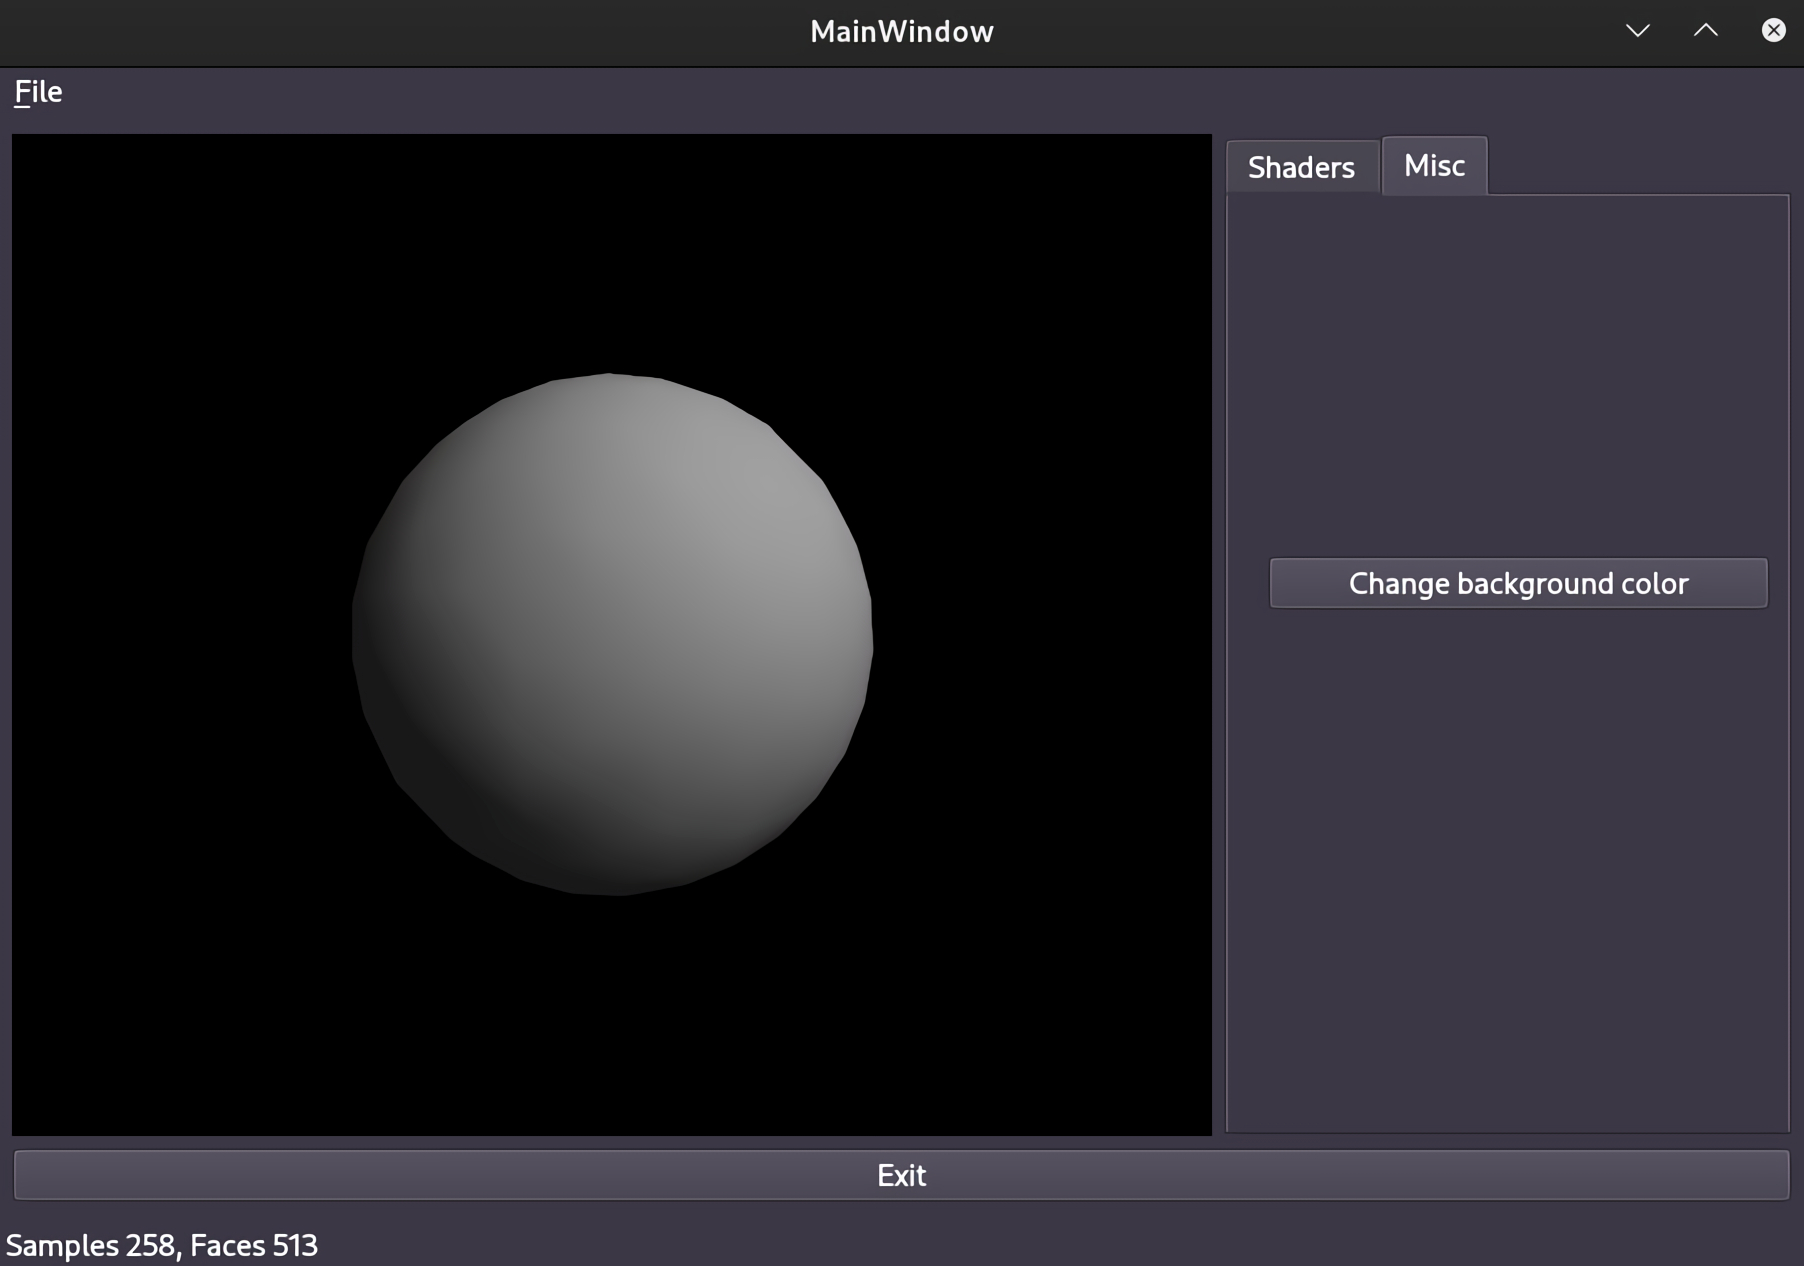
\includegraphics[width=.4\textwidth]{Interface.jpg}
    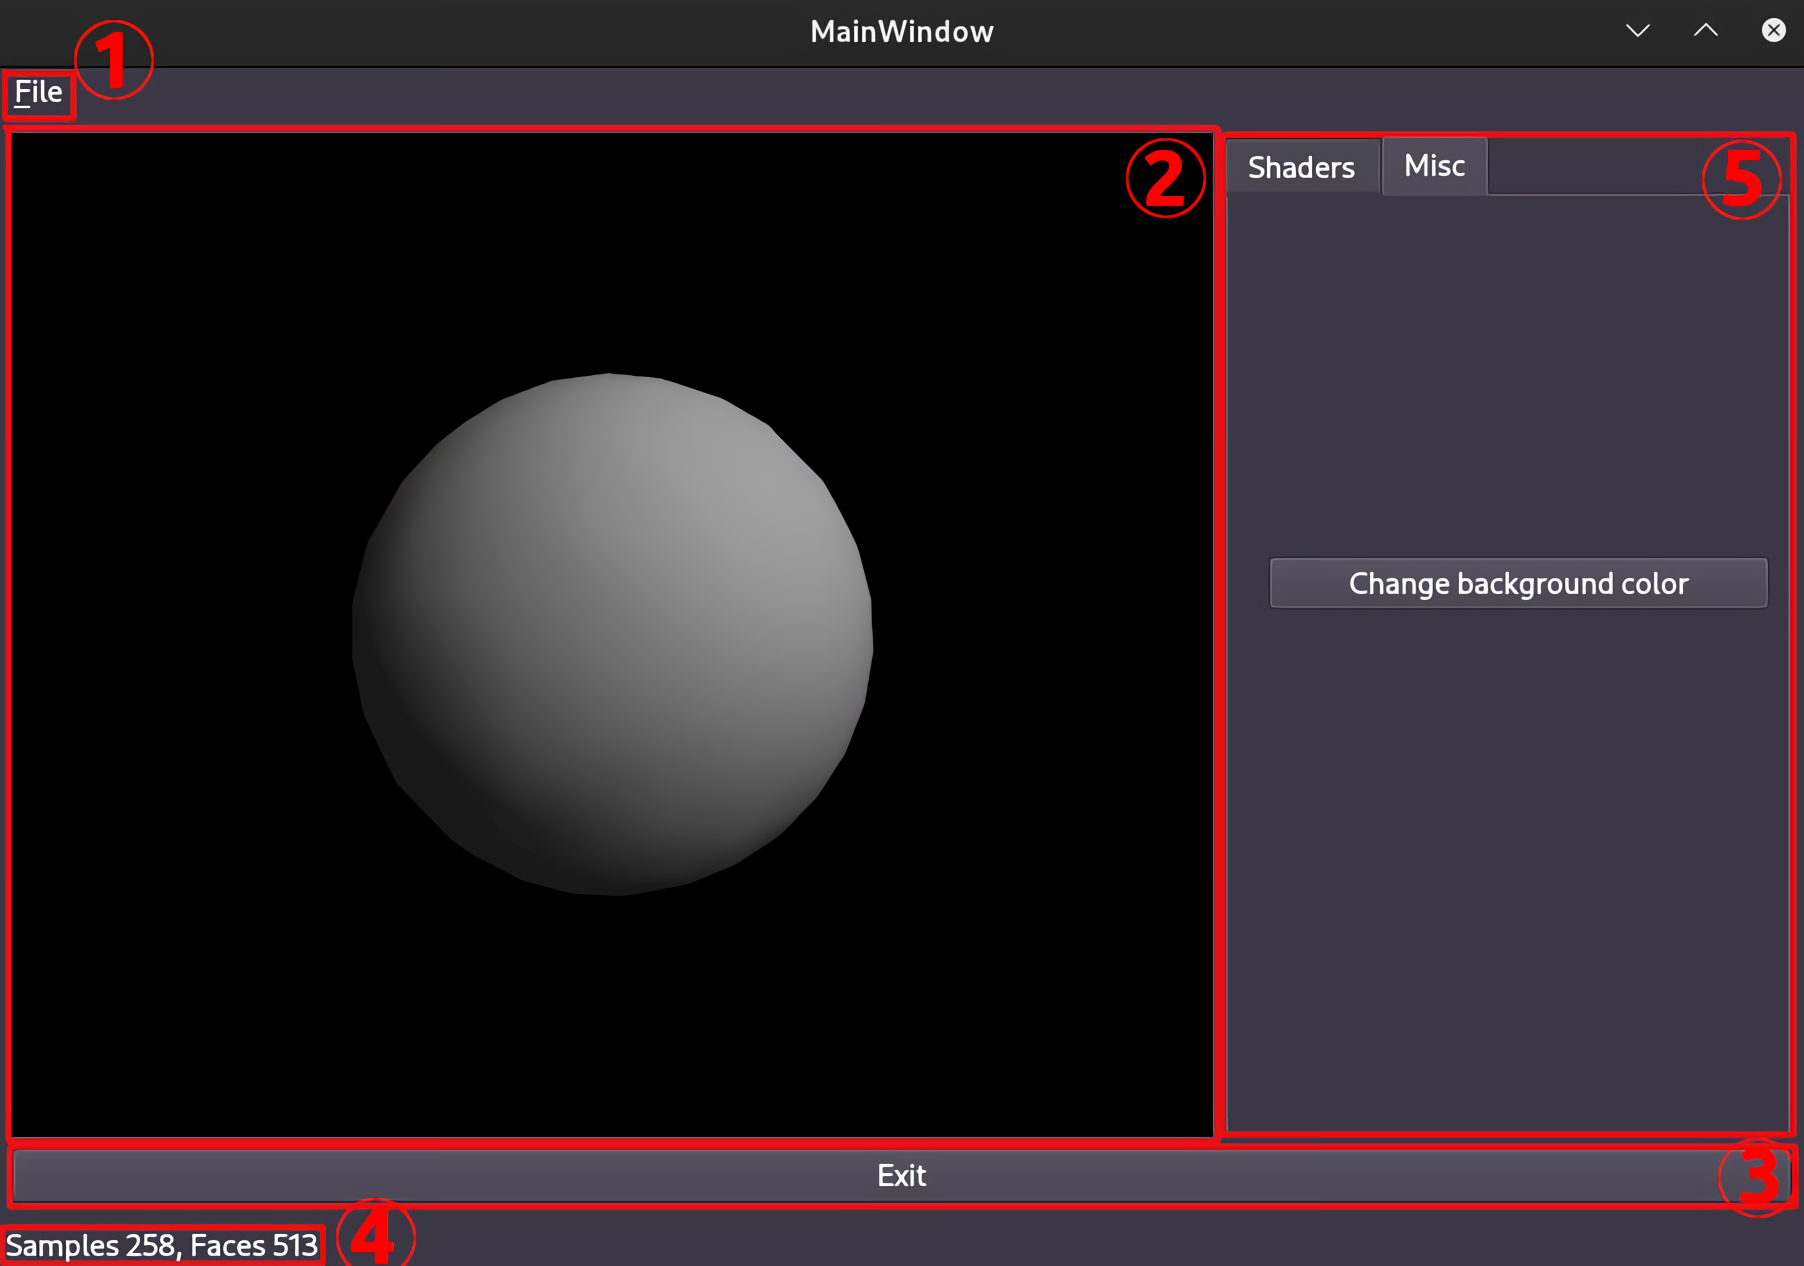
\includegraphics[width=.4\textwidth]{Interfacemarcada.jpg}
    \caption{À esquerda temos a principal interface do programa e ao lado temos a mesma interface
    com marcações para sinalizar os principais componentes.}
\end{figure}

A área de interação do Qt é composta de Widgets, desde os botões, até o canvas 
do OpenGL, todos os elementos são Widgets que podem ser dimensionados na tela e 
mais importante, podem usar sinais para comunicar entre-si.

\subsubsection{File}

Primeiro temos o QMenuBar responsável em expandir e mostrar as duas
opções presentes:

\begin{itemize}
    \item \textbf{Open} - O primeiro QMenu possui um QAction, um sinal conectado
    com o visualizador dos objetos (GLWidget). Quando acionado (triggered) realiza
    a ação de abrir o gerenciador de arquivos e abrir um arquivo .off.
    \item \textbf{Screenshot} - O outro QMenu possui um QAction que conecta 
    ao GLWidget. Quando acionado (triggered) realiza a ação de abrir o gerenciador de arquivos
    e permite o usuário salvar o frame atual do GLWidget como uma imagem png.
\end{itemize}

\begin{figure}[H]
    \centering
    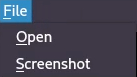
\includegraphics[width=.2\textwidth]{File.jpg}
    \caption{O botão \textbf{File} expandido}
\end{figure}

Além disso, o QMenuBar possui \textbf{Keybinds}, atalhos do teclado do usuário, 
que permitem que todas as iterações com o QMenuBar sejam mais rápidas. Eis a seguir 
os keybinds implementados:

\begin{itemize}
    \item \textbf{Alt + f} $\rightarrow$ clicar no botão \emph{File}
    \begin{itemize}
        \item \textbf{Alt + f + o} $\rightarrow$ abrir um arquivo 
        \item \textbf{Alt + f + s} $\rightarrow$ salvar uma captura de tela 
    \end{itemize}
\end{itemize}

\newpage

\subsubsection{Visualizador de Objetos 3D}

O principal componente da aplicação, a janela onde os objetos 3D 
são exibidos é um GLWidget, em que há grande parte da implementação da 
API do OpenGL.

Esta janela ilustra o resultado final do processamento dos objetos, com texturas e shaders, se necessário.
Além de capturar as teclas do teclado e o movimento do mouse.


\begin{figure}[H]
    \centering
    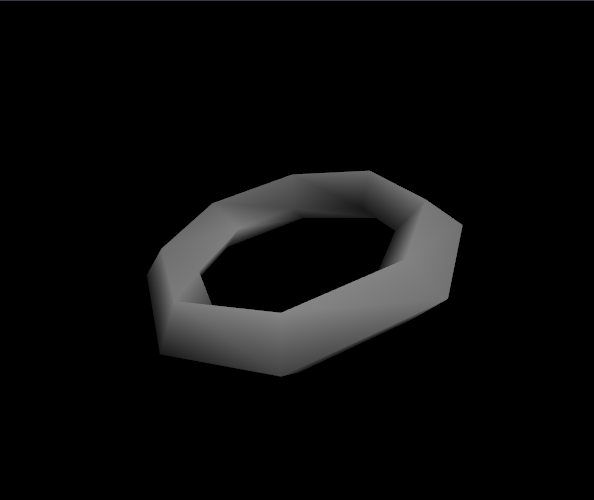
\includegraphics[width=.5\textwidth]{opengl.png}
    \caption{Objeto \textbf{octtorus.off} sendo exibido na janela}
\end{figure}

As possíveis entradas de teclado na aplicação são:

\textbf{Teclado:}

\begin{itemize}
    \item \textbf{Número 1 do teclado} $\rightarrow$ aplicar o algoritmo de \emph{Gouraud}
    \item \textbf{Número 2 do teclado} $\rightarrow$ aplicar o algoritmo de \emph{Phong}
    \item \textbf{Número 3 do teclado} $\rightarrow$ aplicar uma textura
    \item \textbf{Número 4 do teclado} $\rightarrow$ aplicar uma textura com normal
    \item \textbf{Esc} $\rightarrow$ fechar a aplicação
\end{itemize}

\textbf{Mouse:}

\begin{itemize}
    \item \textbf{Scroll} - Realizar ampliação/distanciamento (zoom) no objeto 
    atualmente selecionado. 
    \item \textbf{Botão direito + movimentar o mouse} - Rotacionar o objeto.
\end{itemize}

\subsubsection{Botão de saída}

QPushButton é um widget que possui um sinal ligado a janela principal do programa,
ao ser clicado fechará a aplicação.

\begin{figure}[H]
    \centering
    
\includegraphics[width=\textwidth]{botao-saida.png}
    \caption{Botão para sair do programa}
\end{figure}

\subsubsection{Barra de status}

A barra de status fica no canto inferior da tela 
informando usuários de quantos \emph{samples} e \emph{faces} foram carregadas 
do objeto 3D.
Esse possui um sinal ligado ao GLWidget, que recebe 
uma QString com as informações mencionadas.

\begin{figure}[H]
    \centering
    
\includegraphics[width=.3\textwidth]{status-bar.png}
    \caption{Barra de status com informações do \textbf{octtorus.off}}
\end{figure}

\newpage

\subsubsection{Abas de edição}

\begin{figure}[H]
    \centering
    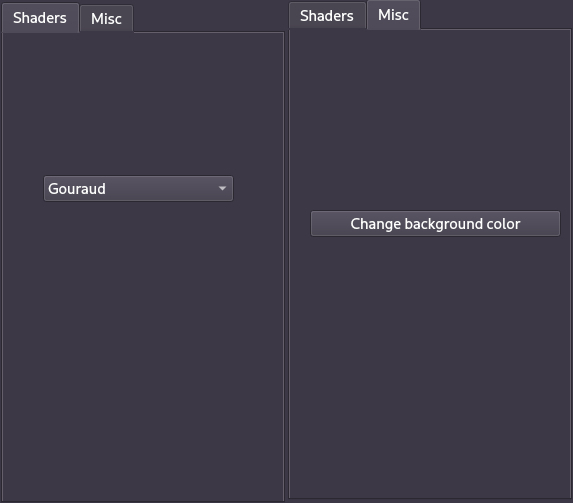
\includegraphics[width=.5\textwidth]{abadeedicao.jpg}
    \caption{As duas abas de edição}
\end{figure}

-------------------------
Para armazenar as possíveis, utilizamos um gerenciador 
de abas (QTabWidget), que armazenará duas abas(QWidget): uma 
responsável em guardar operações com shaders, e outra 
para trocar cor do fundo do GLWidget.
-------------------------

\begin{itemize}
    \item \textbf{Shaders} - Possui um QComboBox, que apresenta 
    vários textos com nome dos possíveis shaders do 
    programa. Após selecionar um, será acionado um sinal 
    que será enviado para o GLWidget pedindo para mudar 
    para o shader especificado pelo usuário.
    \item \textbf{Misc} - Possui um QPushButton, que acionará a 
    paleta de cor do Qt, permitindo que o usuário escolha 
    uma cor para ser a nova cor do fundo (mais informações 
    na seção do código).
\end{itemize}